\documentclass[tikz,border=2pt]{standalone}
\usepackage{amsmath,amssymb}
\usepackage{tikz}
\usetikzlibrary{arrows.meta}

\begin{document}
% Pencils: y* = 6000, D = 100 per day, t0 = 60 days, lead time L = 12 days: the order must be
% placed when the stock falls to DL = 1200, twelve days before it would run out.
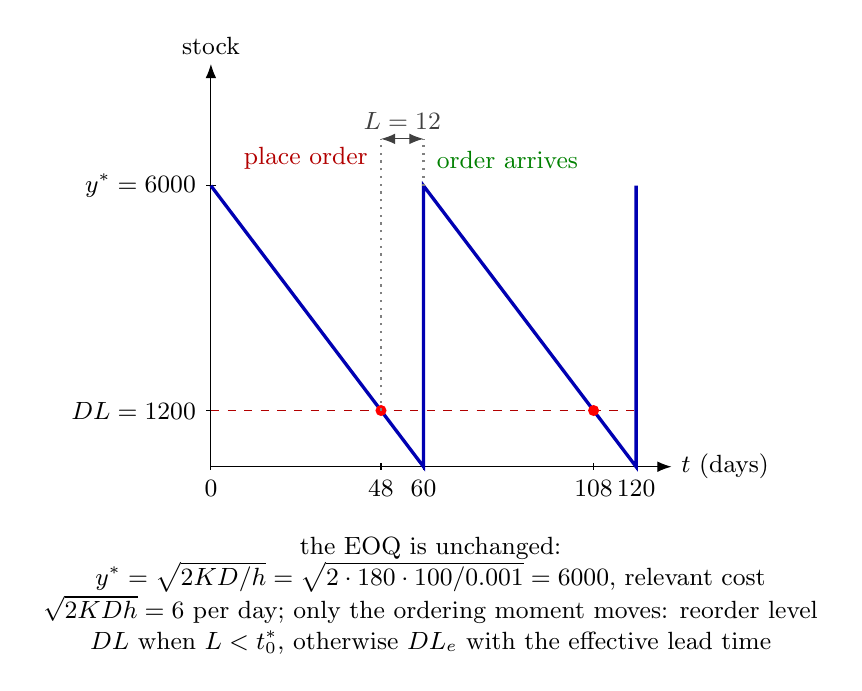
\begin{tikzpicture}[every node/.style={font=\small}, >={Latex[length=1.8mm]}, x=0.045cm, y=0.0006cm]
	\draw[->] (0,0) -- (130,0) node[right, font=\small] {$t$ (days)};
	\draw[->] (0,0) -- (0,8600) node[above, font=\small] {stock};
	\foreach \t in {0,48,60,108,120} {\draw (\t,80) -- (\t,-80) node[below, font=\small] {$\t$};}
	\draw (1.5,6000) -- (-1.5,6000) node[left, font=\small] {$y^*=6000$};
	\draw (1.5,1200) -- (-1.5,1200) node[left, font=\small] {$DL=1200$};
	\draw[blue!70!black, very thick] (0,6000) -- (60,0) -- (60,6000) -- (120,0) -- (120,6000);
	\draw[red!70!black, dashed] (0,1200) -- (120,1200);
	\fill[red] (48,1200) circle (2pt); \fill[red] (108,1200) circle (2pt);
	\draw[gray, dotted, thick] (48,1200) -- (48,7000);
	\draw[gray, dotted, thick] (60,6000) -- (60,7000);
	\draw[<->, gray!50!black] (48,7000) -- (60,7000) node[midway, above, font=\small] {$L=12$};
	\node[red!70!black, font=\small, anchor=south east] at (47,6150) {place order};
	\node[green!50!black, font=\small, anchor=south west] at (61,6150) {order arrives};
	\node[anchor=north, align=flush center, text width=10cm] at (62,-1300) {the EOQ is unchanged: $y^\ast=\sqrt{2KD/h}=\sqrt{2\cdot180\cdot100/0.001}=6000$, relevant cost $\sqrt{2KDh}=6$ per day; only the ordering moment moves: reorder level $DL$ when $L<t_0^\ast$, otherwise $DL_e$ with the effective lead time};
\end{tikzpicture}
\end{document}
